\documentclass[twoside]{book}

% Packages required by doxygen
\usepackage{calc}
\usepackage{doxygen}
\usepackage{graphicx}
\usepackage[utf8]{inputenc}
\usepackage{makeidx}
\usepackage{multicol}
\usepackage{multirow}
\usepackage{textcomp}
\usepackage[table]{xcolor}

% Font selection
\usepackage[T1]{fontenc}
\usepackage{mathptmx}
\usepackage[scaled=.90]{helvet}
\usepackage{courier}
\usepackage{amssymb}
\usepackage{sectsty}
\renewcommand{\familydefault}{\sfdefault}
\allsectionsfont{%
  \fontseries{bc}\selectfont%
  \color{darkgray}%
}
\renewcommand{\DoxyLabelFont}{%
  \fontseries{bc}\selectfont%
  \color{darkgray}%
}

% Page & text layout
\usepackage{geometry}
\geometry{%
  a4paper,%
  top=2.5cm,%
  bottom=2.5cm,%
  left=2.5cm,%
  right=2.5cm%
}
\tolerance=750
\hfuzz=15pt
\hbadness=750
\setlength{\emergencystretch}{15pt}
\setlength{\parindent}{0cm}
\setlength{\parskip}{0.2cm}
\makeatletter
\renewcommand{\paragraph}{%
  \@startsection{paragraph}{4}{0ex}{-1.0ex}{1.0ex}{%
    \normalfont\normalsize\bfseries\SS@parafont%
  }%
}
\renewcommand{\subparagraph}{%
  \@startsection{subparagraph}{5}{0ex}{-1.0ex}{1.0ex}{%
    \normalfont\normalsize\bfseries\SS@subparafont%
  }%
}
\makeatother

% Headers & footers
\usepackage{fancyhdr}
\pagestyle{fancyplain}
\fancyhead[LE]{\fancyplain{}{\bfseries\thepage}}
\fancyhead[CE]{\fancyplain{}{}}
\fancyhead[RE]{\fancyplain{}{\bfseries\leftmark}}
\fancyhead[LO]{\fancyplain{}{\bfseries\rightmark}}
\fancyhead[CO]{\fancyplain{}{}}
\fancyhead[RO]{\fancyplain{}{\bfseries\thepage}}
\fancyfoot[LE]{\fancyplain{}{}}
\fancyfoot[CE]{\fancyplain{}{}}
\fancyfoot[RE]{\fancyplain{}{\bfseries\scriptsize Generated on Wed Mar 26 2014 12:10:14 for ECS by Doxygen }}
\fancyfoot[LO]{\fancyplain{}{\bfseries\scriptsize Generated on Wed Mar 26 2014 12:10:14 for ECS by Doxygen }}
\fancyfoot[CO]{\fancyplain{}{}}
\fancyfoot[RO]{\fancyplain{}{}}
\renewcommand{\footrulewidth}{0.4pt}
\renewcommand{\chaptermark}[1]{%
  \markboth{#1}{}%
}
\renewcommand{\sectionmark}[1]{%
  \markright{\thesection\ #1}%
}

% Indices & bibliography
\usepackage{natbib}
\usepackage[titles]{tocloft}
\setcounter{tocdepth}{3}
\setcounter{secnumdepth}{5}
\makeindex

% Hyperlinks (required, but should be loaded last)
\usepackage{ifpdf}
\ifpdf
  \usepackage[pdftex,pagebackref=true]{hyperref}
\else
  \usepackage[ps2pdf,pagebackref=true]{hyperref}
\fi
\hypersetup{%
  colorlinks=true,%
  linkcolor=blue,%
  citecolor=blue,%
  unicode%
}

% Custom commands
\newcommand{\clearemptydoublepage}{%
  \newpage{\pagestyle{empty}\cleardoublepage}%
}


%===== C O N T E N T S =====

\begin{document}

% Titlepage & ToC
\hypersetup{pageanchor=false}
\pagenumbering{roman}
\begin{titlepage}
\vspace*{7cm}
\begin{center}%
{\Large E\-C\-S \\[1ex]\large 0.\-9 }\\
\vspace*{1cm}
{\large Generated by Doxygen 1.8.4}\\
\vspace*{0.5cm}
{\small Wed Mar 26 2014 12:10:14}\\
\end{center}
\end{titlepage}
\clearemptydoublepage
\tableofcontents
\clearemptydoublepage
\pagenumbering{arabic}
\hypersetup{pageanchor=true}

%--- Begin generated contents ---
\chapter{Hierarchical Index}
\section{Class Hierarchy}
This inheritance list is sorted roughly, but not completely, alphabetically\-:\begin{DoxyCompactList}
\item \contentsline{section}{E\-C\-S\-:\-:Private\-:\-:Component\-Base}{\pageref{class_e_c_s_1_1_private_1_1_component_base}}{}
\begin{DoxyCompactList}
\item \contentsline{section}{E\-C\-S\-:\-:Component$<$ T $>$}{\pageref{class_e_c_s_1_1_component}}{}
\end{DoxyCompactList}
\item \contentsline{section}{E\-C\-S\-:\-:Entity\-Manager}{\pageref{class_e_c_s_1_1_entity_manager}}{}
\item \contentsline{section}{E\-C\-S\-:\-:Entity\-Observer}{\pageref{class_e_c_s_1_1_entity_observer}}{}
\begin{DoxyCompactList}
\item \contentsline{section}{E\-C\-S\-:\-:System\-Manager}{\pageref{class_e_c_s_1_1_system_manager}}{}
\end{DoxyCompactList}
\item \contentsline{section}{E\-C\-S\-:\-:Entity\-System}{\pageref{class_e_c_s_1_1_entity_system}}{}
\item \contentsline{section}{E\-C\-S\-:\-:Private\-:\-:Internal\-Entity}{\pageref{struct_e_c_s_1_1_private_1_1_internal_entity}}{}
\end{DoxyCompactList}

\chapter{Class Index}
\section{Class List}
Here are the classes, structs, unions and interfaces with brief descriptions\-:\begin{DoxyCompactList}
\item\contentsline{section}{\hyperlink{class_e_c_s_1_1_component}{E\-C\-S\-::\-Component$<$ T $>$} \\*A component is a collection of data that can be associated with an entity }{\pageref{class_e_c_s_1_1_component}}{}
\item\contentsline{section}{\hyperlink{class_e_c_s_1_1_private_1_1_component_base}{E\-C\-S\-::\-Private\-::\-Component\-Base} \\*Private type. Keeps track of type I\-Ds and allow for component polymorphism }{\pageref{class_e_c_s_1_1_private_1_1_component_base}}{}
\item\contentsline{section}{\hyperlink{class_e_c_s_1_1_entity_manager}{E\-C\-S\-::\-Entity\-Manager} \\*Manages all entities and components in the world }{\pageref{class_e_c_s_1_1_entity_manager}}{}
\item\contentsline{section}{\hyperlink{class_e_c_s_1_1_entity_observer}{E\-C\-S\-::\-Entity\-Observer} \\*Can be inherited from to observe additions/removal of entities and components }{\pageref{class_e_c_s_1_1_entity_observer}}{}
\item\contentsline{section}{\hyperlink{class_e_c_s_1_1_entity_system}{E\-C\-S\-::\-Entity\-System} \\*An entity system base class }{\pageref{class_e_c_s_1_1_entity_system}}{}
\item\contentsline{section}{\hyperlink{struct_e_c_s_1_1_private_1_1_internal_entity}{E\-C\-S\-::\-Private\-::\-Internal\-Entity} }{\pageref{struct_e_c_s_1_1_private_1_1_internal_entity}}{}
\item\contentsline{section}{\hyperlink{class_e_c_s_1_1_system_manager}{E\-C\-S\-::\-System\-Manager} \\*Management class for entity systems }{\pageref{class_e_c_s_1_1_system_manager}}{}
\end{DoxyCompactList}

\chapter{Class Documentation}
\hypertarget{class_e_c_s_1_1_component}{\section{E\-C\-S\-:\-:Component$<$ T $>$ Class Template Reference}
\label{class_e_c_s_1_1_component}\index{E\-C\-S\-::\-Component$<$ T $>$@{E\-C\-S\-::\-Component$<$ T $>$}}
}


A component is a collection of data that can be associated with an entity.  




{\ttfamily \#include $<$component.\-h$>$}

Inheritance diagram for E\-C\-S\-:\-:Component$<$ T $>$\-:\begin{figure}[H]
\begin{center}
\leavevmode
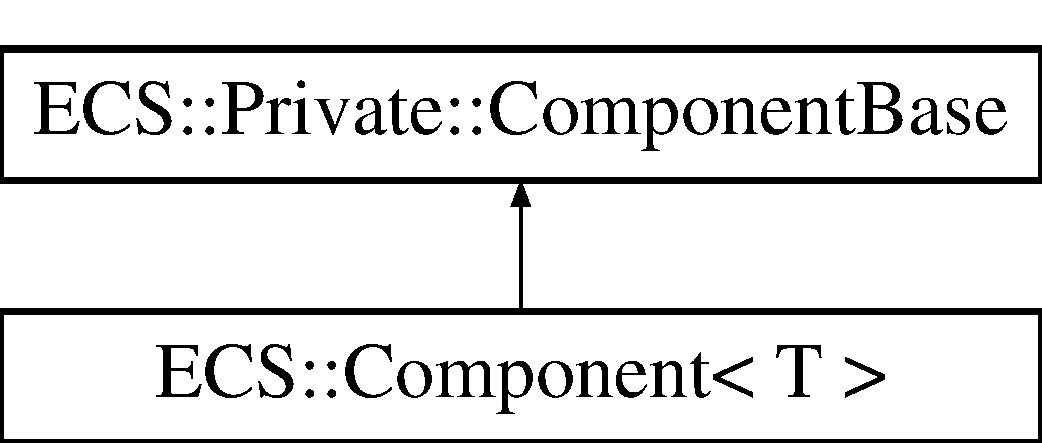
\includegraphics[height=2.000000cm]{class_e_c_s_1_1_component}
\end{center}
\end{figure}
\subsection*{Static Public Attributes}
\begin{DoxyCompactItemize}
\item 
\hypertarget{class_e_c_s_1_1_component_a5ffc2d06fe6e84e6bcf14956cae79b79}{static const int \hyperlink{class_e_c_s_1_1_component_a5ffc2d06fe6e84e6bcf14956cae79b79}{I\-D} = Private\-::\-Component\-Base\-::next\-Type\-Id++}\label{class_e_c_s_1_1_component_a5ffc2d06fe6e84e6bcf14956cae79b79}

\begin{DoxyCompactList}\small\item\em Type I\-D for the component. This is increased automatically for every instantiated type of the class. \end{DoxyCompactList}\end{DoxyCompactItemize}
\subsection*{Protected Member Functions}
\begin{DoxyCompactItemize}
\item 
\hypertarget{class_e_c_s_1_1_component_a91e0d98831c5692ba752b1233fd01b24}{\hyperlink{class_e_c_s_1_1_component_a91e0d98831c5692ba752b1233fd01b24}{Component} ()}\label{class_e_c_s_1_1_component_a91e0d98831c5692ba752b1233fd01b24}

\begin{DoxyCompactList}\small\item\em Protected constructor. Only inherited classes can be instantiated. \end{DoxyCompactList}\end{DoxyCompactItemize}


\subsection{Detailed Description}
\subsubsection*{template$<$typename T$>$class E\-C\-S\-::\-Component$<$ T $>$}

A component is a collection of data that can be associated with an entity. 

Inherit from this class to create your own component types. Pass along the inherited type as the template parameter. 

The documentation for this class was generated from the following file\-:\begin{DoxyCompactItemize}
\item 
ecs/include/component.\-h\end{DoxyCompactItemize}

\hypertarget{class_e_c_s_1_1_private_1_1_component_base}{\section{E\-C\-S\-:\-:Private\-:\-:Component\-Base Class Reference}
\label{class_e_c_s_1_1_private_1_1_component_base}\index{E\-C\-S\-::\-Private\-::\-Component\-Base@{E\-C\-S\-::\-Private\-::\-Component\-Base}}
}


Private type. Keeps track of type I\-Ds and allow for component polymorphism.  




{\ttfamily \#include $<$component.\-h$>$}

Inheritance diagram for E\-C\-S\-:\-:Private\-:\-:Component\-Base\-:\begin{figure}[H]
\begin{center}
\leavevmode
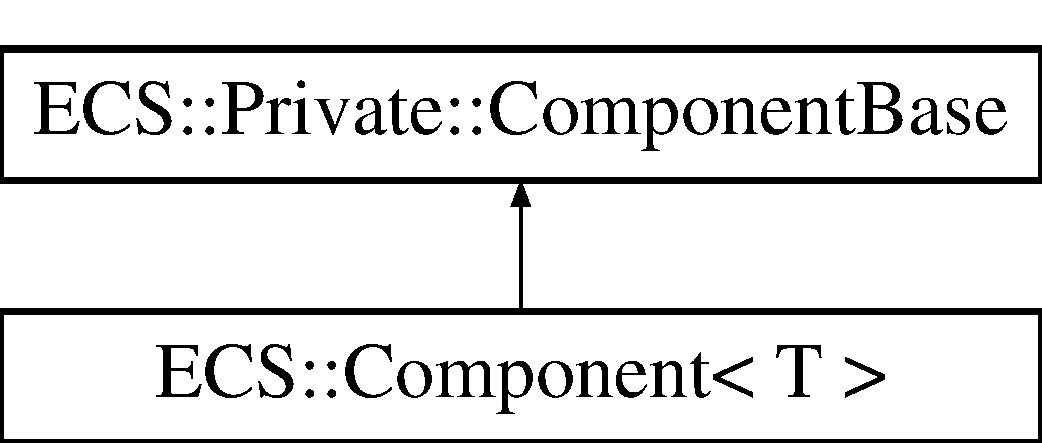
\includegraphics[height=2.000000cm]{class_e_c_s_1_1_private_1_1_component_base}
\end{center}
\end{figure}
\subsection*{Protected Member Functions}
\begin{DoxyCompactItemize}
\item 
\hypertarget{class_e_c_s_1_1_private_1_1_component_base_a29d60cb01485127847456183e204b167}{\hyperlink{class_e_c_s_1_1_private_1_1_component_base_a29d60cb01485127847456183e204b167}{Component\-Base} ()}\label{class_e_c_s_1_1_private_1_1_component_base_a29d60cb01485127847456183e204b167}

\begin{DoxyCompactList}\small\item\em Protected constructor. Only inherited classes can be instantiated. \end{DoxyCompactList}\end{DoxyCompactItemize}
\subsection*{Friends}
\begin{DoxyCompactItemize}
\item 
\hypertarget{class_e_c_s_1_1_private_1_1_component_base_a8201bf3780452dd2c643fdd6bdf77155}{{\footnotesize template$<$typename T $>$ }\\class {\bfseries E\-C\-S\-::\-Component}}\label{class_e_c_s_1_1_private_1_1_component_base_a8201bf3780452dd2c643fdd6bdf77155}

\end{DoxyCompactItemize}


\subsection{Detailed Description}
Private type. Keeps track of type I\-Ds and allow for component polymorphism. 

The documentation for this class was generated from the following files\-:\begin{DoxyCompactItemize}
\item 
ecs/include/component.\-h\item 
ecs/src/component.\-cpp\end{DoxyCompactItemize}

\hypertarget{class_e_c_s_1_1_entity_manager}{\section{E\-C\-S\-:\-:Entity\-Manager Class Reference}
\label{class_e_c_s_1_1_entity_manager}\index{E\-C\-S\-::\-Entity\-Manager@{E\-C\-S\-::\-Entity\-Manager}}
}


Manages all entities and components in the world.  




{\ttfamily \#include $<$entitymanager.\-h$>$}

\subsection*{Public Member Functions}
\begin{DoxyCompactItemize}
\item 
\hypertarget{class_e_c_s_1_1_entity_manager_a2b65211b0059901010486bcbedd84b96}{{\bfseries Entity\-Manager} (size\-\_\-t reserved\-Entity\-Count=R\-E\-S\-E\-R\-V\-E\-D\-\_\-\-E\-N\-T\-I\-T\-Y\-\_\-\-C\-O\-U\-N\-T)}\label{class_e_c_s_1_1_entity_manager_a2b65211b0059901010486bcbedd84b96}

\item 
Entity \hyperlink{class_e_c_s_1_1_entity_manager_a58a521f1a18027231d2895cf91a6b555}{Create\-Entity} ()
\begin{DoxyCompactList}\small\item\em Creates an entity without components. \end{DoxyCompactList}\item 
void \hyperlink{class_e_c_s_1_1_entity_manager_ae3c584bf9245a3dcbafc1cc5ea93b642}{Remove\-Entity} (Entity entity)
\begin{DoxyCompactList}\small\item\em Marks an entity and its components for removal and removes it from all systems. \end{DoxyCompactList}\item 
{\footnotesize template$<$typename T $>$ }\\T $\ast$ \hyperlink{class_e_c_s_1_1_entity_manager_a735ab328f07b45342c392fe1f1b6f925}{Add\-Component} (Entity entity)
\begin{DoxyCompactList}\small\item\em Create a component and add it to the entity. \end{DoxyCompactList}\item 
{\footnotesize template$<$typename T $>$ }\\T $\ast$ \hyperlink{class_e_c_s_1_1_entity_manager_a7ee27d400563107f222693fb103c21ed}{Get\-Component} (Entity entity)
\begin{DoxyCompactList}\small\item\em Get the component of type T on entity. \end{DoxyCompactList}\item 
{\footnotesize template$<$typename T $>$ }\\void \hyperlink{class_e_c_s_1_1_entity_manager_a78ee8abb53ca6a324496ea839503ac3f}{Remove\-Component} (Entity entity)
\begin{DoxyCompactList}\small\item\em Mark a component for removal and remove its flag from the entity. \end{DoxyCompactList}\end{DoxyCompactItemize}


\subsection{Detailed Description}
Manages all entities and components in the world. 

\subsection{Member Function Documentation}
\hypertarget{class_e_c_s_1_1_entity_manager_a735ab328f07b45342c392fe1f1b6f925}{\index{E\-C\-S\-::\-Entity\-Manager@{E\-C\-S\-::\-Entity\-Manager}!Add\-Component@{Add\-Component}}
\index{Add\-Component@{Add\-Component}!ECS::EntityManager@{E\-C\-S\-::\-Entity\-Manager}}
\subsubsection[{Add\-Component}]{\setlength{\rightskip}{0pt plus 5cm}template$<$typename T $>$ T $\ast$ E\-C\-S\-::\-Entity\-Manager\-::\-Add\-Component (
\begin{DoxyParamCaption}
\item[{Entity}]{entity}
\end{DoxyParamCaption}
)}}\label{class_e_c_s_1_1_entity_manager_a735ab328f07b45342c392fe1f1b6f925}


Create a component and add it to the entity. 

Template type T is the concrete type of the component.

\begin{DoxyReturn}{Returns}
The created component. 
\end{DoxyReturn}
\hypertarget{class_e_c_s_1_1_entity_manager_a58a521f1a18027231d2895cf91a6b555}{\index{E\-C\-S\-::\-Entity\-Manager@{E\-C\-S\-::\-Entity\-Manager}!Create\-Entity@{Create\-Entity}}
\index{Create\-Entity@{Create\-Entity}!ECS::EntityManager@{E\-C\-S\-::\-Entity\-Manager}}
\subsubsection[{Create\-Entity}]{\setlength{\rightskip}{0pt plus 5cm}Entity E\-C\-S\-::\-Entity\-Manager\-::\-Create\-Entity (
\begin{DoxyParamCaption}
{}
\end{DoxyParamCaption}
)}}\label{class_e_c_s_1_1_entity_manager_a58a521f1a18027231d2895cf91a6b555}


Creates an entity without components. 

\begin{DoxyReturn}{Returns}
The created entity. 
\end{DoxyReturn}
\hypertarget{class_e_c_s_1_1_entity_manager_a7ee27d400563107f222693fb103c21ed}{\index{E\-C\-S\-::\-Entity\-Manager@{E\-C\-S\-::\-Entity\-Manager}!Get\-Component@{Get\-Component}}
\index{Get\-Component@{Get\-Component}!ECS::EntityManager@{E\-C\-S\-::\-Entity\-Manager}}
\subsubsection[{Get\-Component}]{\setlength{\rightskip}{0pt plus 5cm}template$<$typename T $>$ T $\ast$ E\-C\-S\-::\-Entity\-Manager\-::\-Get\-Component (
\begin{DoxyParamCaption}
\item[{Entity}]{entity}
\end{DoxyParamCaption}
)}}\label{class_e_c_s_1_1_entity_manager_a7ee27d400563107f222693fb103c21ed}


Get the component of type T on entity. 

\begin{DoxyReturn}{Returns}
\hyperlink{class_e_c_s_1_1_component}{Component} or nullptr if no component of type T exists on the entity. 
\end{DoxyReturn}
\hypertarget{class_e_c_s_1_1_entity_manager_a78ee8abb53ca6a324496ea839503ac3f}{\index{E\-C\-S\-::\-Entity\-Manager@{E\-C\-S\-::\-Entity\-Manager}!Remove\-Component@{Remove\-Component}}
\index{Remove\-Component@{Remove\-Component}!ECS::EntityManager@{E\-C\-S\-::\-Entity\-Manager}}
\subsubsection[{Remove\-Component}]{\setlength{\rightskip}{0pt plus 5cm}template$<$typename T $>$ void E\-C\-S\-::\-Entity\-Manager\-::\-Remove\-Component (
\begin{DoxyParamCaption}
\item[{Entity}]{entity}
\end{DoxyParamCaption}
)}}\label{class_e_c_s_1_1_entity_manager_a78ee8abb53ca6a324496ea839503ac3f}


Mark a component for removal and remove its flag from the entity. 

Template type T is the concrete type of the component. This function will also remove the entity from all relevant systems. \hypertarget{class_e_c_s_1_1_entity_manager_ae3c584bf9245a3dcbafc1cc5ea93b642}{\index{E\-C\-S\-::\-Entity\-Manager@{E\-C\-S\-::\-Entity\-Manager}!Remove\-Entity@{Remove\-Entity}}
\index{Remove\-Entity@{Remove\-Entity}!ECS::EntityManager@{E\-C\-S\-::\-Entity\-Manager}}
\subsubsection[{Remove\-Entity}]{\setlength{\rightskip}{0pt plus 5cm}void E\-C\-S\-::\-Entity\-Manager\-::\-Remove\-Entity (
\begin{DoxyParamCaption}
\item[{Entity}]{entity}
\end{DoxyParamCaption}
)}}\label{class_e_c_s_1_1_entity_manager_ae3c584bf9245a3dcbafc1cc5ea93b642}


Marks an entity and its components for removal and removes it from all systems. 

This function will remove the entity from the processing list of all systems. It will not recycle or remove its components however; this will be done after the current system is finished processing. 

The documentation for this class was generated from the following files\-:\begin{DoxyCompactItemize}
\item 
ecs/include/entitymanager.\-h\item 
ecs/src/entitymanager.\-cpp\end{DoxyCompactItemize}

\hypertarget{class_e_c_s_1_1_entity_system}{\section{E\-C\-S\-:\-:Entity\-System Class Reference}
\label{class_e_c_s_1_1_entity_system}\index{E\-C\-S\-::\-Entity\-System@{E\-C\-S\-::\-Entity\-System}}
}


An entity system base class.  




{\ttfamily \#include $<$system.\-h$>$}

\subsection*{Public Member Functions}
\begin{DoxyCompactItemize}
\item 
\hypertarget{class_e_c_s_1_1_entity_system_a9f67d3f6c3b997a164665f1a36e19f0d}{void \hyperlink{class_e_c_s_1_1_entity_system_a9f67d3f6c3b997a164665f1a36e19f0d}{Process} ()}\label{class_e_c_s_1_1_entity_system_a9f67d3f6c3b997a164665f1a36e19f0d}

\begin{DoxyCompactList}\small\item\em Process all entities matching the set aspect. \end{DoxyCompactList}\item 
virtual void \hyperlink{class_e_c_s_1_1_entity_system_a5f2443358fcbe4ddd7c2bfb46d75cd86}{Process\-Entity} (Entity entity)=0
\begin{DoxyCompactList}\small\item\em Process one of the entities in our processing list. \end{DoxyCompactList}\item 
\hypertarget{class_e_c_s_1_1_entity_system_ab5bd1ebaeab36edbe5619110bfb469fd}{const std\-::bitset\\*
$<$ M\-A\-X\-\_\-\-C\-O\-M\-P\-O\-N\-E\-N\-T\-S $>$ \& \hyperlink{class_e_c_s_1_1_entity_system_ab5bd1ebaeab36edbe5619110bfb469fd}{Get\-Aspect} () const }\label{class_e_c_s_1_1_entity_system_ab5bd1ebaeab36edbe5619110bfb469fd}

\begin{DoxyCompactList}\small\item\em Get the aspect of the system. \end{DoxyCompactList}\end{DoxyCompactItemize}
\subsection*{Friends}
\begin{DoxyCompactItemize}
\item 
\hypertarget{class_e_c_s_1_1_entity_system_ab1ef2aa9992dd8ae85793e1a1f980e1e}{class {\bfseries System\-Manager}}\label{class_e_c_s_1_1_entity_system_ab1ef2aa9992dd8ae85793e1a1f980e1e}

\end{DoxyCompactItemize}


\subsection{Detailed Description}
An entity system base class. 

An entity system will process entities that have a list of components that matches the aspect of the system.

To start using a system, it has to be added to a \hyperlink{class_e_c_s_1_1_system_manager}{System\-Manager} that is associated to an \hyperlink{class_e_c_s_1_1_entity_manager}{Entity\-Manager}. 

\subsection{Member Function Documentation}
\hypertarget{class_e_c_s_1_1_entity_system_a5f2443358fcbe4ddd7c2bfb46d75cd86}{\index{E\-C\-S\-::\-Entity\-System@{E\-C\-S\-::\-Entity\-System}!Process\-Entity@{Process\-Entity}}
\index{Process\-Entity@{Process\-Entity}!ECS::EntitySystem@{E\-C\-S\-::\-Entity\-System}}
\subsubsection[{Process\-Entity}]{\setlength{\rightskip}{0pt plus 5cm}virtual void E\-C\-S\-::\-Entity\-System\-::\-Process\-Entity (
\begin{DoxyParamCaption}
\item[{Entity}]{entity}
\end{DoxyParamCaption}
)\hspace{0.3cm}{\ttfamily [pure virtual]}}}\label{class_e_c_s_1_1_entity_system_a5f2443358fcbe4ddd7c2bfb46d75cd86}


Process one of the entities in our processing list. 

This function is called for every entity matching our aspect when Process is called.


\begin{DoxyParams}{Parameters}
{\em entity} & The entity to process. \\
\hline
\end{DoxyParams}


The documentation for this class was generated from the following files\-:\begin{DoxyCompactItemize}
\item 
ecs/include/system.\-h\item 
ecs/src/system.\-cpp\end{DoxyCompactItemize}

\hypertarget{struct_e_c_s_1_1_private_1_1_internal_entity}{\section{E\-C\-S\-:\-:Private\-:\-:Internal\-Entity Struct Reference}
\label{struct_e_c_s_1_1_private_1_1_internal_entity}\index{E\-C\-S\-::\-Private\-::\-Internal\-Entity@{E\-C\-S\-::\-Private\-::\-Internal\-Entity}}
}
\subsection*{Public Attributes}
\begin{DoxyCompactItemize}
\item 
\hypertarget{struct_e_c_s_1_1_private_1_1_internal_entity_a5e74b188dffd2aee52d0a4f1259eb140}{std\-::bitset$<$ M\-A\-X\-\_\-\-C\-O\-M\-P\-O\-N\-E\-N\-T\-S $>$ \hyperlink{struct_e_c_s_1_1_private_1_1_internal_entity_a5e74b188dffd2aee52d0a4f1259eb140}{flags}}\label{struct_e_c_s_1_1_private_1_1_internal_entity_a5e74b188dffd2aee52d0a4f1259eb140}

\begin{DoxyCompactList}\small\item\em Defines what components are associated with this entity. \end{DoxyCompactList}\end{DoxyCompactItemize}


The documentation for this struct was generated from the following file\-:\begin{DoxyCompactItemize}
\item 
ecs/include/entity.\-h\end{DoxyCompactItemize}

\hypertarget{class_e_c_s_1_1_system_manager}{\section{E\-C\-S\-:\-:System\-Manager Class Reference}
\label{class_e_c_s_1_1_system_manager}\index{E\-C\-S\-::\-System\-Manager@{E\-C\-S\-::\-System\-Manager}}
}


Management class for entity systems.  




{\ttfamily \#include $<$systemmanager.\-h$>$}

\subsection*{Public Member Functions}
\begin{DoxyCompactItemize}
\item 
void \hyperlink{class_e_c_s_1_1_system_manager_a429f0b17229926adea3315c736232e7d}{Register\-System} (\hyperlink{class_e_c_s_1_1_entity_system}{Entity\-System} $\ast$system)
\begin{DoxyCompactList}\small\item\em Registers a system within the manager. \end{DoxyCompactList}\end{DoxyCompactItemize}


\subsection{Detailed Description}
Management class for entity systems. 

This manager will keep track of all existing entity systems and update their processing list. 

\subsection{Member Function Documentation}
\hypertarget{class_e_c_s_1_1_system_manager_a429f0b17229926adea3315c736232e7d}{\index{E\-C\-S\-::\-System\-Manager@{E\-C\-S\-::\-System\-Manager}!Register\-System@{Register\-System}}
\index{Register\-System@{Register\-System}!ECS::SystemManager@{E\-C\-S\-::\-System\-Manager}}
\subsubsection[{Register\-System}]{\setlength{\rightskip}{0pt plus 5cm}void E\-C\-S\-::\-System\-Manager\-::\-Register\-System (
\begin{DoxyParamCaption}
\item[{{\bf Entity\-System} $\ast$}]{system}
\end{DoxyParamCaption}
)}}\label{class_e_c_s_1_1_system_manager_a429f0b17229926adea3315c736232e7d}


Registers a system within the manager. 

This will transfer control of the system from the user to the manager. The manager will delete it later.


\begin{DoxyParams}{Parameters}
{\em system} & A heap-\/allocated entity system. \\
\hline
\end{DoxyParams}


The documentation for this class was generated from the following file\-:\begin{DoxyCompactItemize}
\item 
ecs/include/systemmanager.\-h\end{DoxyCompactItemize}

%--- End generated contents ---

% Index
\newpage
\phantomsection
\addcontentsline{toc}{part}{Index}
\printindex

\end{document}
